\section{Выполнение программы}

\subsection{Загрузка программы}

Программа открывается как веб-страница, либо как index.html файл в комплекте поставки.

\subsection{Выполнение программы}

После открытия страницы в браузере, пользователь должен выбрать на своем устройстве .json файл экспорта из Telegram.

\begin{figure}[h!]
    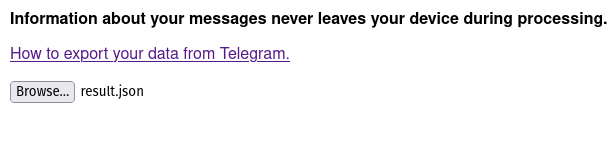
\includegraphics[width=\linewidth]{ro/img/upload.png}
    \caption{Интерфейс загрузки .JSON-файла}
    \label{fig:upload}
\end{figure}


После загрузки файла, пользователь увидит агрегированную статистику, собранную на данных из файла. 
Она включает в себя имя пользователя, которому принадлежат данные, количество его контактов, и количество пользователей, которые упоминаются в сообщениях.

\begin{figure}[h!]
    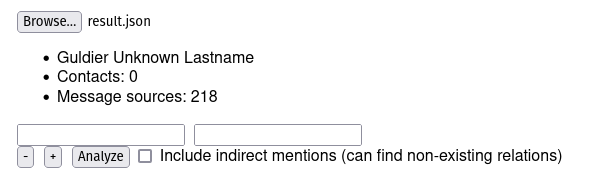
\includegraphics[width=\linewidth]{ro/img/aggregate.png}
    \caption{Пример общей статистики}
    \label{fig:aggregate}
\end{figure}


Для поиска связей в социальном графе пользователю необходимо указать в соответствующих полях имена контактов для поиска. 
Для удобства использования в полях работает автодополнение по всем контактам, встречающимся в наборе данных.

Опционально можно включить опцию "Include indirect mentions". Когда она включена, в граф будет добавлена информация о упоминании одним пользователем имени другого.
По умолчанию она выключена, т.к. имена пользователей Telegram зачастую являются обычными словами (Например, аккаунт с именем "Да."), что приводит к появлению в графе ложных связей.

\begin{figure}[h!]
    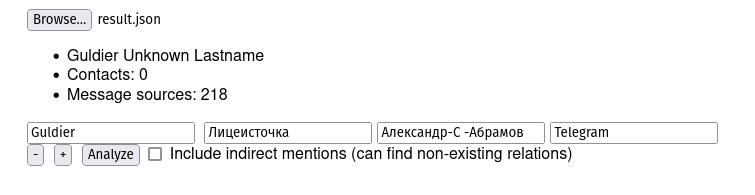
\includegraphics[width=\linewidth]{ro/img/input.png}
    \caption{Интерфейс указания пользователей}
    \label{fig:input}
\end{figure}


После этого пользователь нажатием соответствующей кнопки может построить визуализацию связей контактов.
На визуализации есть легенда, описывающая типы объектов (пользователь, чат, канал, ...).
При необходимости, нажатием на категорию в легенде, можно скрыть соответствующий набор объектов.

Связи между пользователями обозначают упоминание одним пользователем другого, между пользователем и чатом - то, что пользователь в него писал.
При этом если чат - личная переписка, то его название будет соответствовать имени пользователя, с которым она велась.

\begin{figure}[h!]
    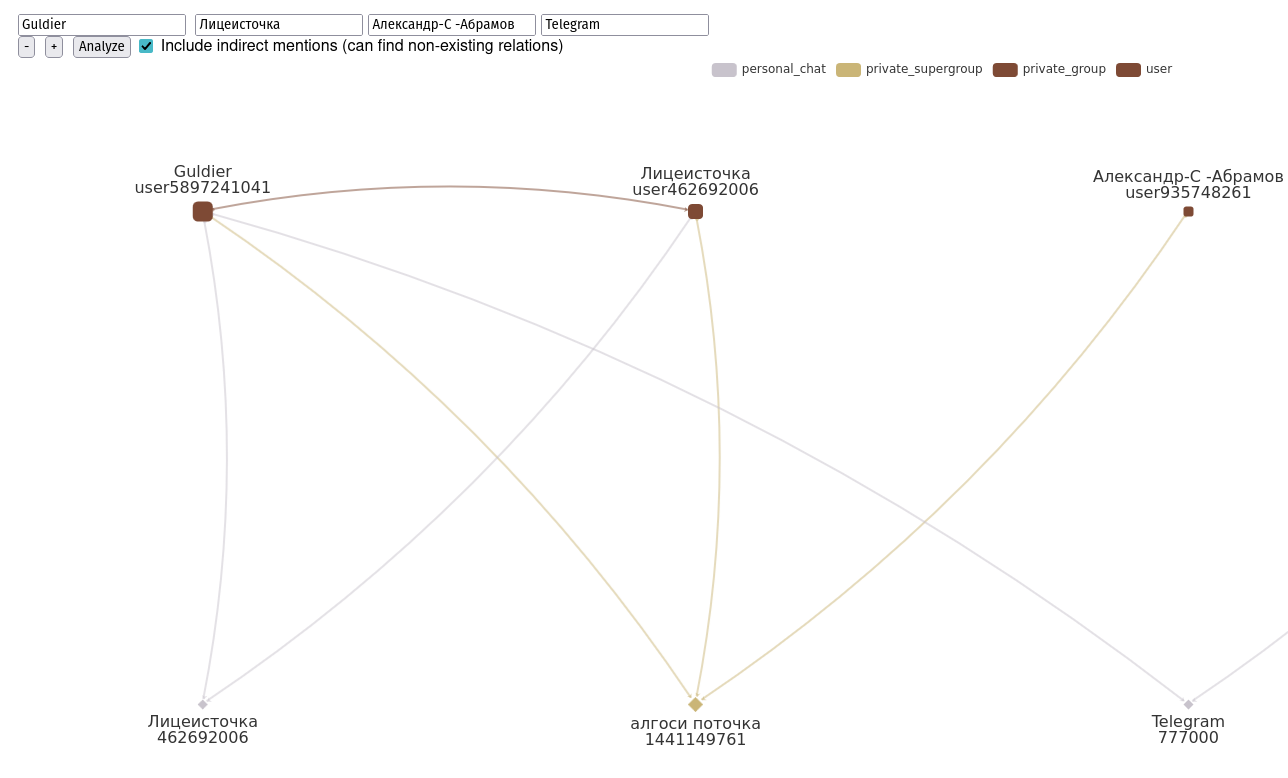
\includegraphics[width=\linewidth]{ro/img/graph.png}
    \caption{Пример построенного графа}
    \label{fig:graph}
\end{figure}